% ---------------------------------------------------------------------------
% When a Safety Layer Stops Being One
% IEEE PES ISGT Asia 2026 -- track: Electric Vehicle-Grid Integration and
% Smart Charging for Carbon Neutrality
%
% Formatted with the conference's own template (IEEE-conference-template-062824,
% IEEEtran) at A4, per the submission requirement. 4-6 pages.
%
% Every number in this manuscript -- in the tables AND in the running text --
% is generated by scripts/make_paper_tables.py from the JSON in results/, and
% every figure by scripts/make_paper_figures.py. Do not type a number into this
% file by hand: a transcription error in a paper passes every check this
% repository runs. In-text figures are the \n... macros from tables/numbers.tex.
%
% Claims are frozen in docs/00-state-of-play.md Sec. 2b. Do not strengthen them
% while drafting -- each is scoped to exactly what was measured, and that
% scoping is what keeps the journal work from contradicting a published
% sentence.
% ---------------------------------------------------------------------------
\documentclass[conference,a4paper]{IEEEtran}
\IEEEoverridecommandlockouts

\usepackage{cite}
\usepackage{amsmath,amssymb,amsfonts}
\usepackage{graphicx}
\usepackage{textcomp}
\usepackage{xcolor}
\usepackage{booktabs}

% generated -- do not edit
\newcommand{\nRecoveryLo}{96.9}
\newcommand{\nRecoveryHi}{100.0}
\newcommand{\nNCells}{12}
\newcommand{\nJacLo}{0.20}
\newcommand{\nJacHi}{5.67}
\newcommand{\nSafeLo}{0.80}
\newcommand{\nSafeHi}{2.06}
\newcommand{\nMvUnderInfeas}{8.3}
\newcommand{\nMvUnderFrozen}{6.9}
\newcommand{\nMvUnderService}{0.7309}
\newcommand{\nMvCorrectService}{0.7698}
\newcommand{\nMvUnderServiceLoss}{3.9}
\newcommand{\nLvOverServiceLoss}{11}
\newcommand{\nLvStaleViol}{0.0642}
\newcommand{\nLvRawViol}{0.0642}
\newcommand{\nLvFreshViol}{0.0000}
\newcommand{\nStaleInfeas}{0.0000}
\newcommand{\nMvCliff}{24}
\newcommand{\nMvCliffEightLo}{3}
\newcommand{\nMvCliffEightHi}{12}
\newcommand{\nLvCliff}{12}
\newcommand{\nServiceRatio}{8.0}
\newcommand{\nGreedyService}{0.7094}
\newcommand{\nLearnedService}{0.0889}
\newcommand{\nTraceDev}{1.4\times 10^{-6}}
\newcommand{\nTraceBelow}{24}
\newcommand{\nTraceSteps}{288}
\newcommand{\nEpisodes}{25}
\newcommand{\nLearnedCells}{6}
\newcommand{\nLearnedSeeds}{3}
\newcommand{\nLearnedRecLo}{97.9}
\newcommand{\nLearnedRecHi}{99.6}
\newcommand{\nSensFast}{0.662}
\newcommand{\nSensSlow}{447.6}


\begin{document}

\title{When a Safety Layer Stops Being One: Base-Point\\ Staleness in
Voltage-Constrained EV Charging
% \thanks{Identify applicable funding agency here. If none, delete this.}
}

\author{\IEEEauthorblockN{Md.\ Rifat Rahman}
\IEEEauthorblockA{\textit{Dept.\ of Electrical and Electronic Engineering} \\
\textit{Bangladesh University of Engineering and Technology}\\
Dhaka, Bangladesh \\
rifatarafat1020@gmail.com}
% TODO: co-authors and affiliations to be settled before submission.
}

\maketitle

\begin{abstract}
Projecting a charging set-point onto a linearised voltage constraint has become
the standard way to make a learned or heuristic controller respect a
distribution feeder's limits. The linearisation has two inputs that are procured
very differently: a Jacobian, computed from a network model, and a base point,
which can only be measured. We separate them on two unrelated radial feeders, a
medium-voltage IEEE 33-bus testbed and a 117-bus low-voltage village benchmark.
A Jacobian wrong by a factor of two costs nothing. A base point that is never
refreshed removes the protection altogether: violations return to within three
percent of the unprojected rate in all twelve cells tested, while the layer
reports no infeasibility whatsoever. The transition is abrupt, and it arrives at
different ages on the two feeders. A second, opposite fault, under-estimated line
impedance, buys a spotless violation record with curtailment. Safety layers need
instrumenting, not outcome-checking.
\end{abstract}

\begin{IEEEkeywords}
Electric vehicle charging, power distribution, reinforcement learning, voltage
control, voltage sensitivity.
\end{IEEEkeywords}

% ===========================================================================
\section{Introduction}
% ===========================================================================

Electrifying road transport moves a large new load onto networks that were never
planned around it. Strong urban distribution absorbs it comfortably. The weak
radial feeders serving rural and semi-rural customers do not: terminal voltage
there begins to sag at low penetration, and the classical remedies---%
reconductoring, a larger transformer, another lateral---are slow, disruptive and
capital-intensive. Buying hosting capacity with control rather than with copper
is therefore an appealing proposition, and it is the premise of most
smart-charging and vehicle-to-grid work aimed at decarbonising transport without
first rebuilding the network beneath it.

Control bought in place of copper needs an assurance attached, because the
operator is now trusting software to keep voltage legal. The prevailing way of
supplying one is a \emph{safety layer}: a small optimisation, sitting between
whatever chooses the set-points and the plant, that takes each request and
returns the nearest request a linearised power-flow model certifies as
admissible~\cite{dalal2018,aamas2023,kou2022,gan2023,bigat2026,evsafe2024}. Its
appeal is that it does not care what sits above it---a trained agent, a tariff
heuristic, a rule---and that it converts a statistical claim about a policy into
a per-step constraint on an action. In the field's own taxonomy of safe
reinforcement learning for power systems, projection of this kind is one of two
techniques within one of the two top-level categories~\cite{saferlreview}.

Underneath the layer sits a linearisation, and that linearisation has two inputs
which the literature almost universally handles as a single object. The
\emph{Jacobian} $\partial V/\partial P$, $\partial V/\partial Q$ describes how
the network responds; obtaining it requires an admittance model, and it changes
only when the network does. The \emph{base point}---the operating condition about
which the Jacobian was taken---describes where the feeder currently is; obtaining
it requires a measurement, and it changes continuously. One can be recomputed
offline as often as one likes. The other cannot be computed at all (Fig.~\ref{fig:loop}).

None of the work cited above reports how often its linearisation is refreshed.
On a transmission system that omission would matter little. On distribution it
matters a great deal: the state-estimation literature describes these networks as
practically unobservable in real time~\cite{dsse_survey}, measurement-scarce,
served by sensors with heterogeneous reporting rates, and easily tipped into
unobservability by a communications fault. Distribution state estimation runs on
cycles of minutes; advanced metering reports on a quarter-hour to an hour. A base
point that is somewhat out of date is not a corner case on a distribution feeder.
It is the ordinary condition.

\begin{figure}[!t]
\centerline{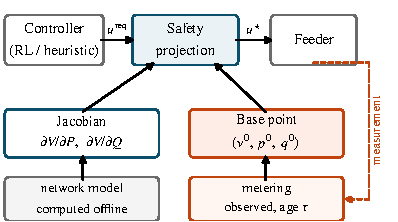
\includegraphics[width=\columnwidth]{figures/fig_loop.pdf}}
\caption{The safety layer has two inputs, procured by different means. The
Jacobian comes from a network model and can be recomputed offline at will; the
base point can only be observed, at whatever cadence the metering provides. This
paper perturbs each independently.}
\label{fig:loop}
\end{figure}

\subsection{What is, and is not, claimed here}

We are explicit about what is not ours. That measurement can substitute for model
accuracy is established in at least three literatures: incremental, sensor-based
flight control replaces model terms with direct measurements and is robust to
model error as a consequence~\cite{indi}; measurement-based (``model-less'')
voltage control estimates sensitivity coefficients from data precisely because
modelled ones are unreliable~\cite{modelless}; and online feedback-based
linearised power flow updates its parameters from instantaneous measurements,
already reporting robustness to measurement error, communication failure and
update rate~\cite{bai2022}. We reconfirm that principle; we do not claim it.

What has not been established is the \emph{closed-loop consequence}. The metric
in~\cite{bai2022} is voltage estimation error, an open-loop measure of accuracy.
Ours is whether the filter still refuses an unsafe action. Neither implies the
other. A model can be badly wrong and still turn away everything dangerous, or
mildly wrong and wave everything through. Accuracy that decays gently does not
entail protection that decays gently---and we find that it does not. Our
contributions are:

\begin{enumerate}
\item \textbf{A silent-failure characterisation.} A never-refreshed projection
      reproduces the unprojected violation rate while reporting zero
      infeasibilities. The failure is total, and it raises no alarm on the
      channel an operator would watch (Sec.~\ref{sec:staleness}).
\item \textbf{A decomposition of the linearisation} into Jacobian and base point,
      each perturbed independently. The half that is expensive to obtain
      tolerates a factor-of-two error; the half constrained by metering carries
      the protection (Sec.~\ref{sec:modelerror}).
\item \textbf{A runtime diagnostic.} Two unrelated faults each produce a clean
      violation rate. We give the telemetry that separates a working layer from
      an absent one (Sec.~\ref{sec:diagnostic}).
\item \textbf{Measured tolerance bands and an operating envelope}, on two feeders
      sharing no topology, voltage level or impedance scale.
\end{enumerate}

We also report, rather than bury, that on these testbeds it is the projection and
not the learned policy that delivers safe service (Sec.~\ref{sec:layer}). That
finding is what turned the study towards the layer instead of the learner, and it
is why a trained agent enters the experiments below as an input to the layer
rather than as the object of study.

% ===========================================================================
\section{Related Work}
% ===========================================================================

\textbf{Safety layers for distribution voltage control.} Dalal \emph{et
al.}~\cite{dalal2018} introduced a layer that analytically corrects an action to
satisfy linearised constraints. The construction has since been carried into
multi-agent voltage control~\cite{aamas2023}, Volt-VAR
optimisation~\cite{kou2022}, communication-delayed inverter
control~\cite{gan2023}, physics-regularised graph learning~\cite{bigat2026} and
EV charging~\cite{evsafe2024}. Two of them take directly opposing positions on
model sensitivity: one advertises that approximate sensitivity information
suffices~\cite{aamas2023}, while another motivates itself by projection being
sensitive to parameter error~\cite{bigat2026}. Neither reports the experiment
that would settle the disagreement. Section~\ref{sec:modelerror} reports it.

\textbf{Sensitivity computation and currency.} Analytic sensitivity coefficients
for radial networks are standard~\cite{christakou2013}. Measurement-based
estimation~\cite{modelless} and online feedback linearisation~\cite{bai2022}
tackle model unavailability head-on. Bai \emph{et al.}~\cite{bai2022} are the
nearest prior work, and the distinction is the one drawn above: they measure how
accurate a linearisation remains, whereas we measure whether a filter built on one still
refuses unsafe actions.

\textbf{Delay and staleness.} Communication delay has been treated as a
millisecond-scale synchronisation problem to be imputed away~\cite{gan2023}. Age
of information has served as a formal staleness metric in power systems, for
transmission-level load frequency control~\cite{aoi_lfc}. We treat hour-scale
base-point age as a design variable for distribution constraint enforcement,
where the failure mode is inertness rather than instability.

% ===========================================================================
\section{The Safety Layer and Its Two Inputs}
% ===========================================================================

\subsection{Feeder and fleet}

A radial feeder carries $N_b$ buses, four of which host bidirectional charging
stations rated $S^{\mathrm{rat}}$. AC power flow is solved at every control step
by a backward--forward sweep validated against Newton--Raphson to
$10^{-9}$\,p.u. The control step is five minutes over a 288-step day. Vehicles
arrive from a bimodal profile with log-normal dwell times and per-vehicle energy
targets, and a station's set-point is shared among its connected vehicles in
proportion to the energy each still owes. We follow the sign convention of the
underlying solver: $p > 0$ is injection into the bus (vehicle-to-grid discharge)
and $p < 0$ is charging. The operational requirement is
$\underline{v} \le v_i \le \overline{v}$ at every bus, with
$[\underline{v}, \overline{v}] = [0.95, 1.05]$\,p.u.

\subsection{The projection}

Let $u = (p^{\mathrm{req}}, q^{\mathrm{req}})$ be the requested station
set-points. The layer returns the admissible point closest to them,
%
\begin{align}
\min_{p,q} \quad & \lVert p - p^{\mathrm{req}} \rVert_2^2
                 + \lVert q - q^{\mathrm{req}} \rVert_2^2 \label{eq:proj}\\
\text{s.t.}\quad
& \underline{v} + \varepsilon \le \hat v(p,q) \le \overline{v} - \varepsilon
  \nonumber\\
& \lVert (p_j, q_j) \rVert_2 \le S^{\mathrm{rat}}_j, \quad
  \lvert p_j - p_j^{-} \rvert \le \Delta^{\max}, \nonumber
\end{align}
%
in which $\varepsilon$ is a tightening margin, $p^{-}$ the previous set-point,
and the predicted voltage is the linearisation
%
\begin{equation}
\hat v(p,q) = \underbrace{v^{0}}_{\text{base point}}
  + \underbrace{\frac{\partial V}{\partial P}}_{\text{Jacobian}}(p - p^{0})
  + \frac{\partial V}{\partial Q}(q - q^{0}).
\label{eq:lin}
\end{equation}
%
Problem~\eqref{eq:proj} is a second-order cone program, solved with CLARABEL
through a parametrisation that is compiled once and re-solved with fresh
parameters each step. A candidate is accepted on its \emph{measured} constraint
residual rather than on the solver's status label, because a hedged-but-feasible
point is common and discarding one freezes stations for nothing.

\subsection{What ages, and what does not}
\label{sec:twohalves}

Equation~\eqref{eq:lin} is the object of this paper. Its two halves are not
merely conceptually distinct; they are procured by different departments, on
different budgets, at different cadences. The Jacobian is a property of the
network. We compute it analytically from a single LU factorisation of the
power-flow Jacobian, in \nSensFast\,ms against \nSensSlow\,ms for finite
differences, so a utility with a model can afford to refresh it as often as it
likes. The base point $(v^{0}, p^{0}, q^{0})$ is a property of the present
operating condition, and no amount of computation will produce one. It has to be
observed.

That asymmetry is why the decomposition is worth making. A designer cannot buy
base-point currency with compute, which is exactly why its requirement needs to
be known before the layer is relied upon. We write $\tau$ for the \emph{base-point
age}: the number of control steps since the linearisation was last taken.
Throughout, ``refresh interval $\tau$'' means the Jacobian and the base point are
both recomputed every $\tau$ steps and held fixed in between, which is what a
controller with periodic state updates does.

\subsection{What happens when the projection fails}

When~\eqref{eq:proj} admits no solution, the station holds its previous
set-point, and after three consecutive failures it latches to zero. We disclose
this rather than defend it: Sec.~\ref{sec:diagnostic} shows the fallback becoming
the dominant mechanism under model error, which is a finding about the design and
not an endorsement of it.

% ===========================================================================
\section{Experimental Setup}
% ===========================================================================

\subsection{Two feeders that share nothing}

Generality cannot be claimed from one set of line impedances, so every result
below is measured on two networks with nothing in common
(Table~\ref{tab:testbeds}). The MV testbed is the IEEE 33-bus Baran--Wu
feeder~\cite{baranwu1989} with a Th\'evenin source impedance $Z_{\mathrm{sub}}$
inserted upstream of the slack bus, giving 34 buses. The LV testbed is the Kerber
\emph{Dorfnetz} German village benchmark~\cite{kerber}: six laterals and 57
households behind a 400\,kVA transformer at 0.4\,kV, with line impedances an
order of magnitude smaller. Both are built in \textsc{pandapower}~\cite{pandapower}.
The LV distribution transformer is folded into an equivalent series line---exact
for a fixed tap---and line shunt capacitance is neglected, which we measured to
shift $V_{\min}$ by $2.2 \times 10^{-5}$\,p.u., three orders of magnitude below
the tightening margin $\varepsilon$.

\begin{table}[!t]
\caption{The Two Testbeds. Nothing Is Shared.}
\label{tab:testbeds}
\centering\small\setlength{\tabcolsep}{3.5pt}
\begin{tabular}{lcc}
\toprule
 & \textbf{MV feeder} & \textbf{LV feeder} \\
\midrule
Base network & IEEE 33-bus (Baran--Wu) & Kerber \emph{Dorfnetz} \\
Buses (incl.\ Th\'evenin) & 34 & 117 \\
Nominal voltage & 12.66\,kV & 0.4\,kV \\
Laterals & 1 trunk + 3 spurs & 6 \\
Load points / total & 32 / 3.72\,MW & 57 / 0.34\,MW \\
Charging stations & 4 $\times$ 80\,kVA & 4 $\times$ 22\,kVA \\
Idle $V_{\min}$ & 0.9658\,p.u. & 0.9686\,p.u. \\
Idle violations & 0.0000 & 0.0000 \\
Uncoordinated violations & 0.0626 & 0.0667 \\
Uncoordinated service & 0.804 & 0.779 \\
\bottomrule
\end{tabular}

\end{table}

\subsection{Operating points chosen by measurement}

An operating point picked for convenience can trivialise a study in either
direction, so both feeders are held to two requirements: the \emph{idle} feeder
must sit strictly inside the band, so that every violation is attributable to a
charging decision, and an uncoordinated charger must break the band, so that the
layer has something to do. On the LV feeder we swept 36 combinations of
substation stiffness, background load and fleet size, then selected the cell
closest to the MV feeder's uncoordinated behaviour on \emph{both} axes at
once---violation rate and service---since a second feeder tuned harder would
inflate the effect and one tuned easier would hide it.

\subsection{Request sources}

A claim about a safety layer should not depend on what feeds it. We therefore
drive the layer from unrelated sources: an uncoordinated greedy charger, a
deadline-aware heuristic that defers non-urgent stations, and, on the MV feeder,
a soft actor--critic agent~\cite{sac} trained under an augmented-Lagrangian cost
constraint over \nLearnedSeeds{} seeds. Three sources are used on the MV feeder
and two on the LV feeder.

\subsection{What we record}

We report the \emph{voltage violation step rate}, the fraction of control steps
at which any bus lies outside the band, and \emph{service}, the fraction of
vehicles meeting their energy target at departure. Just as importantly we report
the layer's own telemetry: the fraction of steps at which~\eqref{eq:proj} was
infeasible, and the fraction at which a station sat latched to zero.
Section~\ref{sec:diagnostic} is about why the first two do not suffice.

Each cell is \nEpisodes{} evaluation episodes on a shared seed band, so that
methods are paired episode by episode. Seeds are derived by hashing run labels,
with disjoint training and evaluation ranges. The implementation carries 90 tests
and reproduces the reference results of the underlying testbed exactly.

% ===========================================================================
\section{Results}
% ===========================================================================

\subsection{The layer, not the learner}
\label{sec:layer}

Before asking what the layer requires, it is worth establishing that the layer,
rather than the policy above it, is what delivers safe service. Projection is
almost always composed with a learned policy, which quietly conflates two
questions: whether the layer makes actions safe, and whether learning adds
anything on top of it. Applying the identical projection to a zero-intelligence
greedy charger separates them (Table~\ref{tab:layer}).

\begin{table}[!t]
\caption{The Same Projection, Different Controllers (MV Feeder)}
\label{tab:layer}
\centering\small\setlength{\tabcolsep}{3.5pt}
\begin{tabular}{lrrrr}
\toprule
Controller & Viol. & Service & Cost & ms/step \\
\midrule
Idle (no charging) & 0.0000 & 0.0000 & \$0 & 1.01 \\
Uncoordinated & 0.0626 & 0.8041 & \$686 & 1.04 \\
IEEE 1547 droop & 0.0000 & 0.0067 & \$63 & 1.04 \\
SafeSAC (learned $+$ proj.) & 0.0000 & 0.0889 & \$255 & --- \\
\textbf{Uncoordinated $+$ proj.} & 0.0000 & 0.7094 & \$595 & 3.10 \\
\bottomrule
\end{tabular}

\end{table}

The projection applied to a controller with no learning at all delivers
\nServiceRatio$\times$ the service of the same projection applied to the trained
agent, at identical zero violations. A sweep over background load and EV
penetration found no cell in which deferring non-urgent stations beat charging
everything: on this testbed deferred energy is never recovered, so the binding
resource is energy over the day rather than its allocation across stations, and
there is no scheduling structure left for a policy to exploit. \emph{This is a
statement about this testbed at this training budget, not a claim that learning
cannot help.} It is why the rest of the paper interrogates the layer, and why the
trained agent appears below only as one request source among three.

\subsection{Ageing the base point}
\label{sec:staleness}

We now hold the network model exactly correct and vary nothing but $\tau$.
Fig.~\ref{fig:cliff} shows every cell normalised by its own unprojected rate, so
that two feeders whose absolute rates differ threefold can be read on one axis;
Table~\ref{tab:staleness} gives the same data in absolute terms, for the
uncoordinated source. Three things stand out.

\begin{table}[!b]
\caption{Violation Step Rate Against Base-Point Age, Uncoordinated Source.
Correct Network Model Throughout. Bold Marks Exactly Zero.}
\label{tab:staleness}
\centering\scriptsize\setlength{\tabcolsep}{2.6pt}
\begin{tabular}{llrrrrrrr}
\toprule
&& \multicolumn{1}{c}{No} & \multicolumn{6}{c}{Base-point refresh interval (control steps)} \\
\cmidrule(lr){3-3}\cmidrule(lr){4-9}
Feeder & $Z_{\mathrm{sub}}$ & proj. & 1 & 3 & 12 & 24 & 48 & 288 \\
\midrule
MV & 6\% & 0.0606 & \textbf{0.0000} & \textbf{0.0000} & \textbf{0.0000} & \textbf{0.0000} & 0.0586 & 0.0606 \\
 & 8\% & 0.1051 & \textbf{0.0000} & \textbf{0.0000} & 0.0001 & 0.0069 & 0.0883 & 0.1051 \\
 & 10\% & 0.1361 & 0.0408 & 0.0413 & 0.0294 & 0.0217 & 0.1058 & 0.1361 \\
\midrule
LV & 1\% & 0.0642 & \textbf{0.0000} & \textbf{0.0000} & \textbf{0.0000} & 0.0015 & 0.0560 & 0.0642 \\
 & 2\% & 0.1206 & \textbf{0.0000} & \textbf{0.0000} & \textbf{0.0000} & 0.0147 & 0.0793 & 0.1206 \\
 & 3\% & 0.2076 & \textbf{0.0000} & \textbf{0.0000} & \textbf{0.0000} & 0.0214 & 0.1178 & 0.2013 \\
\bottomrule
\end{tabular}

\end{table}

\begin{figure}[!t]
\centerline{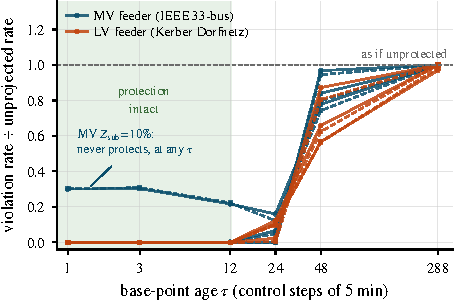
\includegraphics[width=\columnwidth]{figures/fig_cliff.pdf}}
\caption{Violation rate as a fraction of each cell's own unprojected rate, for
twelve cells across two feeders, three substation stiffnesses each and two
request sources. Shading marks the ages at which every cell inside the operating
envelope still holds the band to within $10^{-3}$. The two MV curves that never
reach zero are at a stiffness where projection alone cannot hold the band at any
cadence.}
\label{fig:cliff}
\end{figure}

\textbf{The layer switches off rather than degrading.} At $\tau = 288$---one
refresh per day, which is to say never after the first solve---the violation rate
is the \emph{unprojected} rate, recovering \nRecoveryLo--\nRecoveryHi\,\% of it
across all \nNCells{} cells and both heuristic sources. The trained agent behaves
the same way: \nLearnedRecLo--\nLearnedRecHi\,\% recovery over \nLearnedCells{}
seed-and-stiffness cells. A base point captured on an idle feeder makes the
constraint look slack at every subsequent step, the feasibility pre-check skips
every solve, and each request passes through untouched.

Fig.~\ref{fig:trace} shows this happening within a single episode, which
aggregated rates cannot. The never-refreshed run and the entirely unprojected run
are not merely similar; over the whole day their minimum-voltage trajectories
differ by at most $\nTraceDev$\,p.u., and both spend the same \nTraceBelow{} of
\nTraceSteps{} steps below the limit. The layer is not intermittently failing. It
is absent.

\begin{figure}[!t]
\centerline{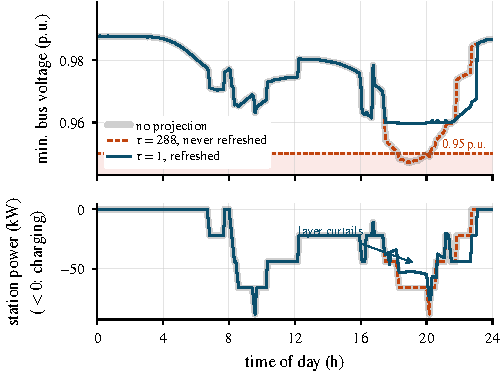
\includegraphics[width=\columnwidth]{figures/fig_trace.pdf}}
\caption{One episode on the LV feeder, three controllers. The never-refreshed
projection (dashed) lies inside the unprojected trace (grey) everywhere, in
voltage and in dispatch alike, while the refreshed projection curtails through
the evening peak and holds the band.}
\label{fig:trace}
\end{figure}

\textbf{It is silent while doing so.} The infeasibility rate at $\tau = 288$ is
\nStaleInfeas{} in every cell. The layer is not failing to solve; it never solves. An
operator watching the component's own fault channel sees nothing at all.

\textbf{The transition is a cliff, and its location is not a constant.} Between
one interval and the next, protection goes from complete to essentially absent.
On the MV feeder the last age at which every cell holds the band exactly is
\nMvCliff{} steps at $Z_{\mathrm{sub}} = 6\,\%$, falling to
\nMvCliffEightLo--\nMvCliffEightHi{} steps at $8\,\%$; on the LV feeder it is
\nLvCliff{} steps at every stiffness tested. We therefore decline to offer a
universal refresh figure. \emph{The cliff exists everywhere we looked; where it
sits varies with the deployment and has to be measured for one.} Nor do we claim
to know what sets it: on the MV feeder it tracks substation stiffness, and on the
LV feeder it does not move at all.

\subsection{Corrupting the model}
\label{sec:modelerror}

We now invert the experiment: the base point is measured on the real feeder at
every step, and only the Jacobian is corrupted, by computing it on a feeder whose
line impedances have been scaled by a factor $k$. This is the arrangement a
deployed controller with an out-of-date network model but live telemetry actually
occupies. Scaling impedances rather than substituting a different feeder keeps
the Jacobian's dimensions matched while moving its magnitude across
\nJacLo$\times$--\nJacHi$\times$ (Fig.~\ref{fig:modelerror}).

\begin{figure}[!t]
\centerline{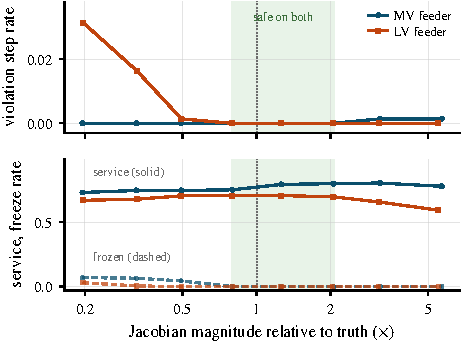
\includegraphics[width=\columnwidth]{figures/fig_model_error.pdf}}
\caption{Violation rate, service and freeze rate against Jacobian magnitude, with
the base point measured every step. Shading marks the window in which violations
are zero on both feeders and both heuristic sources. Under-estimated impedance
costs service through the fallback long before it costs voltage.}
\label{fig:modelerror}
\end{figure}

A Jacobian wrong by up to roughly a factor of two costs nothing: violations are
zero throughout \nSafeLo$\times$--\nSafeHi$\times$ on both feeders and both
heuristic sources. Set against Sec.~\ref{sec:staleness}, the asymmetry is the
paper's central practical point. The half of the linearisation that is expensive
to obtain, and that a distribution utility may simply not possess, tolerates
substantial error. The half that cannot be computed at all carries the
protection.

Outside that window the failure is directional, and which direction is
feeder-dependent: the LV feeder leaks violations when impedance is
under-estimated, the MV feeder when it is over-estimated. Over-estimation is the
conservative side, and it is not free either---on the LV feeder a
$5.5\times$ Jacobian holds violations at zero but costs \nLvOverServiceLoss{}
percentage points of service.

\subsection{Zero is not evidence}
\label{sec:diagnostic}

The two failure modes are mirror images, and Table~\ref{tab:diagnostic} sets them
side by side.

\begin{table}[!t]
\caption{Two Failure Modes. Neither Shows in the Column an Operator Watches.}
\label{tab:diagnostic}
\centering\footnotesize\setlength{\tabcolsep}{3pt}
\begin{tabular}{llrrrr}
\toprule
& Condition & Viol. & Infeas. & Frozen & Service \\
\midrule
LV & Correct model, refreshed hourly & 0.0000 & 0.0000 & 0.0000 & 0.7304 \\
LV & Base point never refreshed & 0.0642 & 0.0000 & 0.0000 & 0.7535 \\
MV & Correct model, refreshed every step & 0.0000 & 0.0016 & 0.0000 & 0.7698 \\
MV & Jacobian under-estimated $5\times$ & 0.0000 & 0.0833 & 0.0694 & 0.7309 \\
\bottomrule
\end{tabular}

\end{table}

A stale base point yields a clean \emph{infeasibility} rate while the feeder goes
entirely unprotected; on the LV feeder the never-refreshed row and the
no-projection row are the same number, \nLvStaleViol{}, to four decimal places.
An under-estimated impedance yields a clean \emph{violation} rate---on the MV
feeder exactly zero, apparently perfect---while the projection is infeasible on
\nMvUnderInfeas\,\% of steps and the fallback has latched stations to zero on
\nMvUnderFrozen\,\%, at a cost of \nMvUnderServiceLoss{} percentage points of
service. In that second case the layer is not protecting the feeder. It is
switching the load off, and being credited for the result.

Neither condition is detectable from the outcome alone. We therefore suggest that
a deployed projection expose, and an operator alarm on, three quantities rather
than one:

\begin{enumerate}
\item \textbf{Base-point age $\tau$}, alarmed against a threshold measured for
      that feeder rather than assumed for it.
\item \textbf{Solve rate.} A projection reporting zero infeasibilities
      \emph{and} a near-zero solve rate on a loaded feeder has stopped binding.
      It is not succeeding; it is absent.
\item \textbf{Fallback activation.} A non-trivial latch rate means the reported
      violation rate was paid for by curtailment rather than by projection.
\end{enumerate}

The first two together amount to a one-line assertion that any of the works in
Sec.~II could adopt at no cost.

\subsection{What it costs to run}

The analytic sensitivity computation takes \nSensFast\,ms against \nSensSlow\,ms
for finite differences, and a full projection step costs a few milliseconds
against a 300\,s control interval---a duty cycle near $0.004\,\%$. Every refresh
interval examined here is computationally free. The constraint on base-point
currency is metering, not computation, which is the practical reading of
Sec.~\ref{sec:modelerror}.

% ===========================================================================
\section{Discussion and Limitations}
% ===========================================================================

\textbf{Scope.} These results are for weak, low-short-circuit-ratio radial
feeders, where voltage rather than thermal loading is the binding constraint. On
robustly built distribution networks the reported voltage impact of EV charging
is small and transformer thermal limits bind first. We make no claim there, and
our testbeds are chosen accordingly.

\textbf{What ``refresh'' means here.} We simulate base-point age by recomputing
the power flow every $\tau$ steps, not by modelling a metering and communication
pipeline. The axis is the \emph{age of the base point}, agnostic to whatever
produces it. Whether real deployments occupy the unsafe region is a question this
paper does not answer; we observe only that the LV feeder's cliff at one hour
coincides with common advanced-metering reporting intervals.

\textbf{Statistics.} We report measured rates over \nEpisodes{} evaluation
episodes per cell and claim no confidence intervals. The effects reported here
are of the form \nLvFreshViol{} against \nLvRawViol{}. The sub-percentage-point
differences we observed between short refresh intervals were of opposite sign on
the two feeders, and we therefore make no claim about them.

\textbf{The fallback.} Freeze-to-zero is a poor fallback, as
Sec.~\ref{sec:diagnostic} makes plain. A layer that curtails to satisfy a
constraint it cannot verify converts a voltage problem into a service problem
without saying so. Designing a fallback that degrades in a declared direction is
open work.

\textbf{Future work.} The natural next step is to make $\tau$ an explicit argument
of the constraint, tightening the band by a data-driven bound on net-load drift
over $\tau$ so that protection degrades continuously instead of switching off.
The construction exists in the control literature for systems with sporadic
measurements~\cite{sporadiccbf}; adapting it to an AC power-flow band, with a
drift bound estimated from measured load rather than assumed adversarial, is
ongoing.

% ===========================================================================
\section{Conclusion}
% ===========================================================================

A sensitivity-based safety layer's protection rests on the currency of its
linearisation base point rather than on the accuracy of its network model. Wrong
by a factor of two, the model costs nothing. A base point that stops being
refreshed removes the protection entirely, reproducing the unprojected violation
rate while reporting no fault, on two feeders that share neither topology nor
voltage level nor impedance scale. The transition is a cliff whose location
varies between deployments, and two distinct faults both present as a clean
number in the column an operator would watch. The remedy is not a faster refresh
rate---every interval examined here is computationally free---but instrumentation:
measure the base-point age, the solve rate and the fallback activation, and alarm
on all three.

% An empty Acknowledgment heading is a defect in a submitted PDF, so the section
% is commented out rather than left standing. Restore it when the text exists.
% \section*{Acknowledgment}
% ...

% Balance the two reference columns on the final page.
\IEEEtriggeratref{10}

\begin{thebibliography}{00}
% NOTE: bibliographic details below are drawn from indexing services and must be
% verified against the papers themselves before submission. Ref. [11] (Bai et
% al.) in particular is the nearest prior work and should be read in full.
%
% Order is first-citation order, as IEEE style requires. If you add, move or
% remove a citation in the body, re-check this ordering -- nothing in the build
% enforces it.

\bibitem{dalal2018} G. Dalal, K. Dvijotham, M. Vecerik, T. Hester, C. Paduraru,
and Y. Tassa, ``Safe exploration in continuous action spaces,'' 2018,
arXiv:1801.08757.

\bibitem{aamas2023} Y. Liu, D. Wu, and X. Wang, ``Multi-agent reinforcement
learning with safety layer for active voltage control,'' in \emph{Proc. Int.
Conf. Autonomous Agents and Multiagent Systems}, 2023, pp. 1533--1541.

\bibitem{kou2022} P. Kou, D. Liang, C. Wang, Z. Wu, and L. Gao,
``Model-augmented safe reinforcement learning for Volt-VAR control in power
distribution networks,'' \emph{Appl. Energy}, vol. 313, p. 118783, 2022.

\bibitem{gan2023} L. Gan, J. Chen, and Y. Zhang, ``Safe multi-agent deep
reinforcement learning for real-time decentralized control of inverter based
renewable energy resources considering communication delay,'' \emph{Appl.
Energy}, vol. 349, p. 121628, 2023.

\bibitem{bigat2026} Y. Zhang and H. Li, ``Physics-regularized and
safety-enhanced Bi-GAT reinforcement learning framework for voltage control,''
\emph{Energies}, vol. 19, no. 2, 2026.

\bibitem{evsafe2024} J. Wang and S. Chen, ``Safety-aware reinforcement learning
for electric vehicle charging station management in distribution network,'' 2024,
arXiv:2403.13236.

\bibitem{saferlreview} X. Chen, G. Qu, and S. Low, ``Safe reinforcement learning
for power system control: A review,'' \emph{Renewable Sustainable Energy Rev.},
vol. 208, 2025.

\bibitem{dsse_survey} K. Dehghanpour, Z. Wang, J. Wang, Y. Yuan, and F. Bu, ``A
survey on state estimation techniques and challenges in smart distribution
systems,'' \emph{IEEE Trans. Smart Grid}, vol. 10, no. 2, pp. 2312--2322, 2019.

\bibitem{indi} P. van Gils, E. van Kampen, C. de Visser, and Q. Chu, ``Stability
and robustness analysis and improvements for incremental nonlinear dynamic
inversion control,'' in \emph{Proc. AIAA Guidance, Navigation, and Control
Conf.}, 2018.

\bibitem{modelless} R. Gupta, F. Sossan, and M. Paolone, ``Model-less robust
voltage control in active distribution networks using sensitivity coefficients
estimated from measurements,'' \emph{Electr. Power Syst. Res.}, vol. 212, 2022.

\bibitem{bai2022} X. Bai, Z. Wang, and Y. Liu, ``An online feedback-based
linearized power flow model for unbalanced distribution networks,'' \emph{IEEE
Trans. Power Syst.}, vol. 37, no. 6, pp. 4600--4611, 2022.

\bibitem{christakou2013} K. Christakou, J.-Y. LeBoudec, M. Paolone, and
D.-C. Tomozei, ``Efficient computation of sensitivity coefficients of node
voltages and line currents in unbalanced radial electrical distribution
networks,'' \emph{IEEE Trans. Smart Grid}, vol. 4, no. 2, pp. 741--750, 2013.

\bibitem{aoi_lfc} M. Zhang and Y. Sun, ``Age-of-information-aware PI controller
for load frequency control,'' \emph{Prot. Control Mod. Power Syst.}, vol. 8,
2023.

\bibitem{baranwu1989} M. E. Baran and F. F. Wu, ``Network reconfiguration in
distribution systems for loss reduction and load balancing,'' \emph{IEEE Trans.
Power Del.}, vol. 4, no. 2, pp. 1401--1407, 1989.

\bibitem{kerber} G. Kerber, ``Aufnahmef\"ahigkeit von
Niederspannungsverteilnetzen f\"ur die Einspeisung aus Photovoltaikkleinanlagen,''
Ph.D. dissertation, Tech. Univ. M\"unchen, Munich, Germany, 2011.

\bibitem{pandapower} L. Thurner, A. Scheidler, F. Sch\"afer, J.-H. Menke,
J. Dollichon, F. Meier, S. Meinecke, and M. Braun, ``pandapower---an open-source
Python tool for convenient modeling, analysis, and optimization of electric power
systems,'' \emph{IEEE Trans. Power Syst.}, vol. 33, no. 6, pp. 6510--6521, 2018.

\bibitem{sac} T. Haarnoja, A. Zhou, P. Abbeel, and S. Levine, ``Soft
actor-critic: Off-policy maximum entropy deep reinforcement learning with a
stochastic actor,'' in \emph{Proc. Int. Conf. Machine Learning}, 2018,
pp. 1861--1870.

\bibitem{sporadiccbf} A. Singletary, Y. Chen, and A. Ames, ``Robust
safety-critical control for systems with sporadic measurements and dwell time
constraints,'' 2024, arXiv:2403.03663.

\end{thebibliography}

\end{document}
